\documentclass[10pt]{article}
% -------------------------------------------------------------------
% Pacotes básicos
\usepackage[english]{babel}										% Idioma a ser usado
                                                                % Trocar "english" para "brazil" para artigos escritos em língua portuguesa 
\usepackage[utf8]{inputenc}										% Escrita de caracteres acentuados e cedilhas - 1
\usepackage[T1]{fontenc}										% Escrita de caracteres acentuados + outros detalhes técnicos fundamentais
% -------------------------------------------------------------------
% Pacotes matemáticos
\usepackage{amsmath,amsfonts,amssymb,amsthm,cancel,siunitx,
calculator,calc,mathtools,empheq,latexsym}
% -------------------------------------------------------------------
% Pacotes para inserção de figuras e subfiguras
\usepackage{subfig,epsfig,tikz,float}		            % Packages de figuras. 
% -------------------------------------------------------------------
% Pacotes para inserção de tabelas
\usepackage{booktabs,multicol,multirow,tabularx,array}          % Packages para tabela
% -------------------------------------------------------------------
\usepackage{float}
\usepackage{biblatex}
\usepackage[colorlinks=true, allcolors=blue]{hyperref}
\usepackage{lipsum}
\usepackage{listings} % for code
% trying to How can one keep a \section from being at the end of a page?
% \usepackage[nobottomtitles*]{titlesec}

% -------------------------------------------------------------------
% Definition of lengths
\setlength{\parskip}{5pt}
\textwidth 13.5cm
\textheight 19.5cm
\columnsep .5cm
% -------------------------------------------------------------------
% Title of the Article
\title{\renewcommand{\baselinestretch}{1.17}\normalsize\bf%
\uppercase{Embedded American Sign Letters Recognition in  Raspberry Pi}
}
% -------------------------------------------------------------------
% Authors
\author{%
João Almeida\\
Joao.SilvadeAlmeida@haw-hamburg.de
}
% -------------------------------------------------------------------

% Begin Document

\begin{document}

\date{}

\maketitle

\vspace{-0.5cm}

\begin{center}
{\footnotesize 
HAW Hamburg, Dept. for Computer Science \\
}
\end{center}

% -------------------------------------------------------------------
% Abstract
\bigskip
\noindent
\begin{abstract}
	Foundation work for training an object detection model with TensorFlow for deployment on an Embedded Raspberry Pi system for recognition of American sign language letters from the camera's obtained video stream. Recognition is done per frame, without considering consecutive frame relations.
%	\lipsum[2-4]
\end{abstract}

\medskip
\noindent
{\small{\bf Keywords}{:} 
computer vision, tensorflow, classification, raspberry pi, python, object detection, machine learning, opencv
}

\baselineskip=\normalbaselineskip

\pagebreak
\tableofcontents
\pagebreak
% -------------------------------------------------------------------

\section{Introduction}\label{sec:1}

	With the increasing reliance on digital technologies for everyday tasks, machines are expected to cover a bigger range of tasks than ever before. Artificial Intelligence is the field of study of what computers can be taught to do, that they couldn't do before. Object detection is a subclass of this field.

	This project provides a proof-of-concept foundation for the application of object detection in the classification of American sign language letters from video obtained by a raspberry pi. 

	The objective is to obtain an accurate prediction, fast and reliably from the limited hardware provided by the raspberry pi.

	\begin{figure}[H]
		\centering
		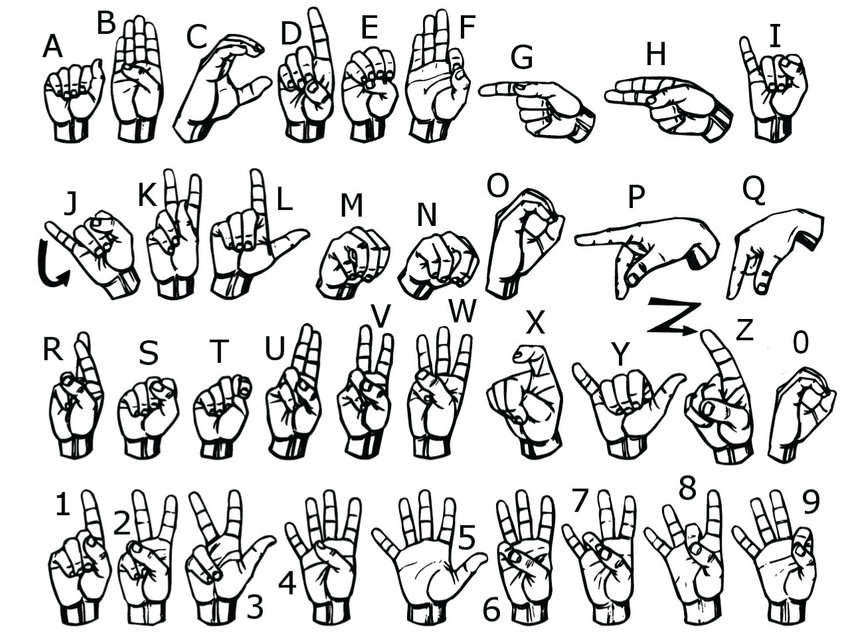
\includegraphics[scale=0.40]{imgs/The-26-letters-and-10-digits-of-American-Sign-Language-ASL.jpg}
		\caption{The 26 letters and 10 digits of American sign language}\label{fig:usage}
	\end{figure}

	\pagebreak

\section{Approach and Architecture}\label{sec:2}

	\subsection{Plan Overview}

		As with any object detection model training process, following the readthedocs official guide for training a custom object detector \cite{1}, the following steps had to be followed:
		\begin{itemize}
			\item Create or obtain an image dataset of letters in american sign language.
			\item Label all the images with information about the position of the hand in the image and the appropriate letter being made.
			\item Train the model with a dedicated graphics card.
			\item Training was done with TensorFlow and the \href{http://download.tensorflow.org/models/object_detection/tf2/20200711/ssd_resnet50_v1_fpn_640x640_coco17_tpu-8.tar.gz}{SSD ResNet50 V1 FPN 640x640} pre-trained model \cite{6}.
			\item Convert the model into a TensorFlow lite model.
			\item Deploy the model in the embedded raspberry pi hardware.
		\end{itemize}

		The training of the model was done in a NVIDIA GeForce RTX 2060 graphics card.

	\subsection{Tools}

		As a means to an end, several architectural choices had to be made, here are some of the tools used:
		\begin{itemize}
			\item As a programming language, python was chosen due to its reputation with the machine learning community and its support for the several methods related to these technologies. More specifically, the language of jupyter notebooks was utilized, allowing for a conjunction of markdown and python code allowing a better structuring of the project.
			\item Conda, the CLI interface for Anaconda, allowing the creation of environments isolated from one another where several machine learning packages could be installed with specific versions, for easier debugging, for the Raspberry Pi OS, the similar tool used for this objective was virtualenv \cite{2}
			\item The machine learning algorithm used was TensorFlow \cite{3}
			\item Due to the large volume of images needed for each letter of the alphabet for a successful classification, in addition to the images obtained and labeled manually, additional images were used from \href{https://public.roboflow.com/object-detection/american-sign-language-letters/1}{this} dataset from roboflow \cite{4}
			\item The main Operating System used was Unix + GNU (Manjaro)
		\end{itemize}

\section{Training and Test Data-set}\label{sec:3}

	The dataset is split into 26 classes, each one representing a letter of the greek alphabet, from $A$ to $Z$.

	As mentioned, a mixed dataset of manually taken photos and already labeled ones from Roboflow\cite{4} has been used.

	\begin{figure}[H]
		\centering
		\begin{minipage}[b]{0.45\textwidth}
			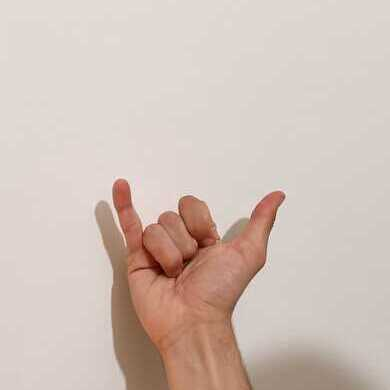
\includegraphics[width=\textwidth]{imgs/Y-m2}
			\caption{Dataset image "Y" - manually gathered}
		\end{minipage}
		\hfill
		\begin{minipage}[b]{0.45\textwidth}
			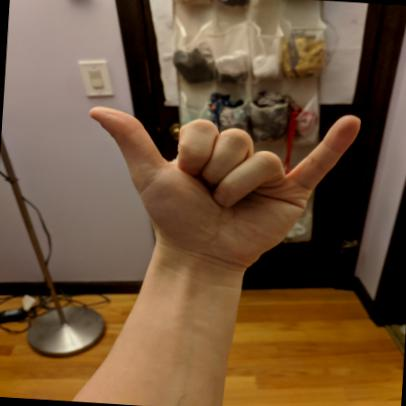
\includegraphics[width=\textwidth]{imgs/training2}
			\caption{Dataset image "Y" - from Roboflow\cite{4}}
		\end{minipage}
	\end{figure}

	The images were gathered with a mobile device, and were downscaled and cropped to 390X390 to be easier to read and speed up the training process. These operations were applied with imagemagick \cite{5} batch commands:

	\begin{lstlisting}[language=bash]
mogrify -resize 390 *.jpeg
mogrify -gravity South -chop 0x267 *.jpeg
mogrify -gravity North -chop 0x206 *.jpeg
	\end{lstlisting}
	
	For the labelling process of the manually gathered images, the program labelImg was used as explained in the \href{https://tensorflow-object-detection-api-tutorial.readthedocs.io/en/latest/training.html#preparing-the-dataset}{readthedocs guide} \cite{1}

	\pagebreak

	\subsection{Image Augmentation}

		Some image augmentation techniques were used as a way to get more dataset images from the manually gathered ones. The ones taken from the internet had already had these techniques applied to them.

		The techniques used for augmentation were horizontal flips of the images, and color conversion to gray scale. The labelling of the new images was done manually for the cases where the bounding box found itself in a different place from the original image.

		\begin{lstlisting}[language=bash]
mogrify -flop *.jpeg # to flip images horizontally
mogrify -colorspace Gray *.jpeg # to greyscale
		\end{lstlisting}

		\begin{figure}[H]
			\centering
			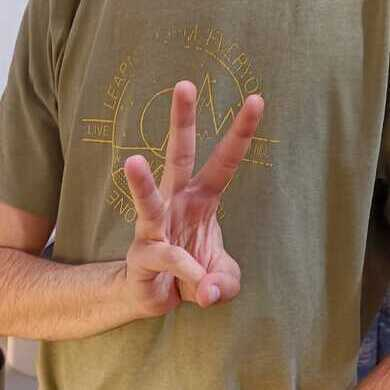
\includegraphics[scale=0.40]{imgs/W-m2.jpeg}
			\caption{Dataset image "W" - Original image}\label{fig:usage}
		\end{figure}

		\begin{figure}[H]
			\centering
			\begin{minipage}[b]{0.40\textwidth}
				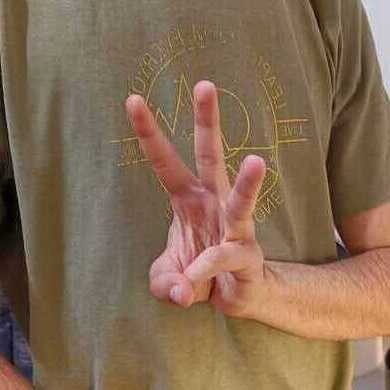
\includegraphics[width=\textwidth]{imgs/W-f2.jpeg}
				\caption{Dataset image "W" - Flipped horizontally}
			\end{minipage}
			\hfill
			\begin{minipage}[b]{0.40\textwidth}
				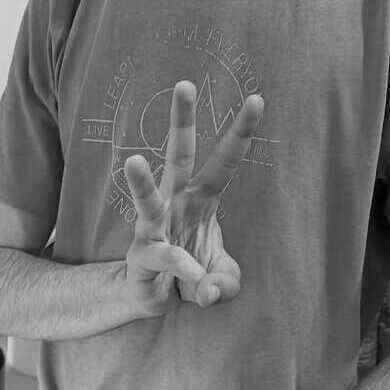
\includegraphics[width=\textwidth]{imgs/W-b2.jpeg}
				\caption{Dataset image "W" - Converted to gray scale}
			\end{minipage}
		\end{figure}

\section{Training Process} 

 	Due to the limited hardware for training, the batch size was decreased to the maximum allowed, without running into the Out Of Memory error. 

	These are some of the more relevant parameters used:
	
	\begin{itemize}
		\item Total images for training: 1668
		\item batch\_size: 4
		\item num\_steps: 25000
		\item The data set was split 90\% for training and 10\% for validation
	\end{itemize}

	As in TensorFlow (without keras) we don't have a direct number for epochs, we can calculate them manually:
	
	$1\ epoch =\frac{Total\ num\ train\ images}{batch\_size} = \frac{1668}{4} = 417\ steps$

	Knowing that 25000 steps were used, and each span of 417 steps represents one epoch, we can calculate the total number of epochs: 
	
	$\frac{25000}{417} = 59.95203836930455 \approx 60$

	Thus, our final epoch count amounts to roughly 60 epochs.

	The loss always decreased steadily indicating a better performance, the learning rate was however not as predictable.

	\begin{figure}[H]
		\centering
		\begin{minipage}[b]{0.45\textwidth}
			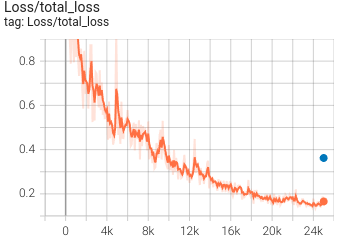
\includegraphics[width=\textwidth]{imgs/total_loss.png}
			\caption{total\_loss}
		\end{minipage}
		\hfill
		\begin{minipage}[b]{0.45\textwidth}
			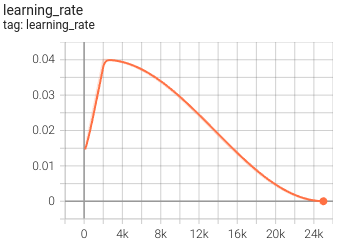
\includegraphics[width=\textwidth]{imgs/learning_rate.png}
			\caption{learning\_rate}
		\end{minipage}
	\end{figure}

	\pagebreak

	\subsection{Testing and Conversion to TFlite}

		Before deployment, it was important to make sure that the model was performing up to standards, for that, \href{https://tensorflow-object-detection-api-tutorial.readthedocs.io/en/latest/auto_examples/object_detection_camera.html#detect-objects-using-your-webcam}{another readthedocs guide was followed} \cite{7} and the laptop's web camera was used to test the model. The following images were obtained:

		\begin{figure}[H]
			\centering
			\begin{minipage}[b]{0.45\textwidth}
				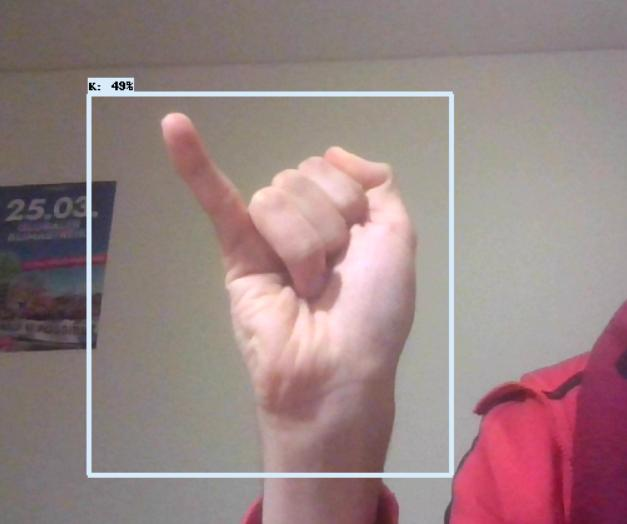
\includegraphics[width=\textwidth]{imgs/myGestures4.jpg}
				\caption{Dataset image "I"}
			\end{minipage}
			\hfill
			\begin{minipage}[b]{0.45\textwidth}
				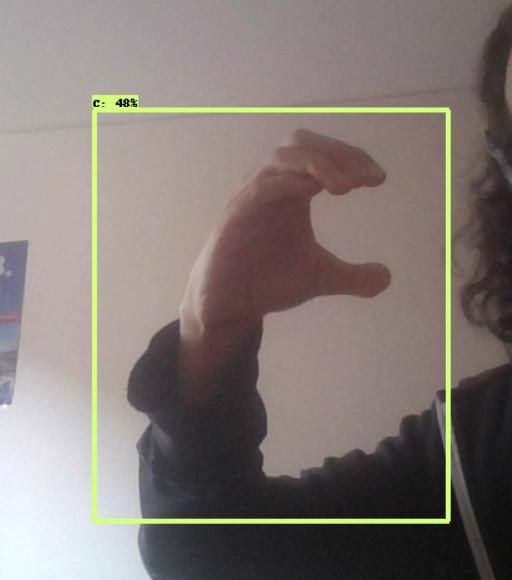
\includegraphics[width=\textwidth]{imgs/myGestures3.jpg}
				\caption{Dataset image "C"}
			\end{minipage}
		\end{figure}

	As for the model conversion to TFlite, in order for it to be able to run on an embedded system, \href{https://colab.research.google.com/github/tensorflow/models/blob/master/research/object_detection/colab_tutorials/convert_odt_model_to_TFLite.ipynb#scrollTo=-ecGLG_Ovjcr}{the linked guide was followed} \cite{8}

	\pagebreak

\section{Deployment on the Raspberry Pi}\label{sec:4}

	

	\subsection{Problems}

		The biggest problems encountered were software wise. 
		
		A new package, picamera2, was used, to be able to communicate with the camera through python, however, for the time being, installing picamera2 is a hassle due to the transition from the legacy camera to the libcamera stack on the raspberry.

		To install it, we needed to build several dependencies, as explained in \href{https://www.raspberrypi.com/news/using-the-picamera2-library-with-tensorflow-lite/}{the raspberry guide followed} \cite{9}

		The installation was successful as it was able to run google's example TFlite model provided.

		\begin{figure}[H]
			\centering
			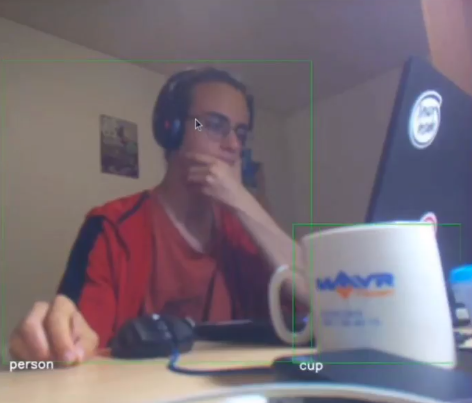
\includegraphics[scale=1]{imgs/RaspberryGoogleModel.png}
			\caption{Google's TFlite example model}\label{fig:usage}
		\end{figure}

	\subsection{Application performance}

		The application was successfully deployed on the Raspberry Pi embedded system by importing the .lite model to the Raspberry Pi after its creation with the guide mentioned above \cite{8}. It had, however, very high latency and its accuracy had decreased massivley, so much so, that in the present state, it would be hard to apply it in any practical environment.

		\pagebreak

\section{Conclusions}\label{sec:5}

	Overall, the project was successful, all the steps of the process were explored and worked on, and the model is able to discern hands from the imagery it receives as input. With it we were able to prove that its possible to run these intricate object detection models even in not very powerful hardware and use them viably.

	The biggest problem is the performance and accuracy of the model, especially once converted into the TFlite version for embedded systems, despite several attempts and guides followed to attempt to successfully convert the model to TFlite\cite{11}\cite{12}, none yielded desireable results, and more time and experimentation would be needed to find a suitable conversion method for the training methods used. Accuracy could likely also be improved with a better conceived dataset and a more thorough training and validating processes. Still, the final outcome of the project is positive as it works as a first increment and building blocks of what could be a much bigger implementation of the idea.

	All project files, libraries used, and several more technical problems faced that were deemed unimportant to tackle in this report can be found in the publicly accessible repository for this project \cite{10}

\newpage

% There is a better way to do the bibliography for sure
\begin{thebibliography}{1}
	\bibitem{1}
	\href{https://tensorflow-object-detection-api-tutorial.readthedocs.io/en/latest/training.html}{Read The Docs. Training Custom Object Detector. (Access date: March 2022) [Online]}
	
	\bibitem{2}
	\href{https://github.com/EdjeElectronics/TensorFlow-Lite-Object-Detection-on-Android-and-Raspberry-Pi/blob/master/Raspberry_Pi_Guide.md#step-1b-download-this-repository-and-create-virtual-environment}{Github. EdjeElectronics. How to Run TensorFlow Lite Object Detection Models on the Raspberry Pi (with Optional Coral USB Accelerator). (Access date: March 2022) [Online]}

	\bibitem{3}
	\href{https://www.tensorflow.org}{TensorFlow. Machine-learning platform. (Access date: March 2022) [Online]}

	\bibitem{4}
	\href{https://public.roboflow.com/object-detection/american-sign-language-letters/1}{Roboflow. American Sign Language Letters Dataset. (Access date: March 2022) [Online]}

	\bibitem{5}
	\href{https://imagemagick.org/index.php}{ImageMagick. (Access date: August 2022) [Online]}

	\bibitem{6}
	\href{https://github.com/tensorflow/models/blob/master/research/object_detection/g3doc/tf2_detection_zoo.md}{Github. TensorFlow 2 Detection Model Zoo. (Access date: March 2022) [Online]}

	\bibitem{7}
	\href{https://tensorflow-object-detection-api-tutorial.readthedocs.io/en/latest/auto_examples/object_detection_camera.html#detect-objects-using-your-webcam}{Read The Docs. Detect Objects Using Your Webcam. (Access date: March 2022) [Online]}

	\bibitem{8}
	\href{https://colab.research.google.com/github/tensorflow/models/blob/master/research/object_detection/colab_tutorials/convert_odt_model_to_TFLite.ipynb#scrollTo=-ecGLG_Ovjcr}{Google Colab. Convert TF Object Detection API model to TFLite. (Access date: March 2022) [Online]}

	\bibitem{9}
	\href{https://www.raspberrypi.com/news/using-the-picamera2-library-with-tensorflow-lite/}{Raspberry Pi. Using the Picamera2 library with TensorFlow Lite. (Access date: March 2022) [Online]}

	\bibitem{10}
	\href{https://github.com/Yeshey/SignLanguageDetection_TenserFlow_RaspberryPi}{Github. SignLanguageDetection\_TenserFlow\_RaspberryPi. [Online]}

	\bibitem{11}
	\href{https://github.com/EdjeElectronics/TensorFlow-Lite-Object-Detection-on-Android-and-Raspberry-Pi}{Github. TensorFlow-Lite-Object-Detection-on-Android-and-Raspberry-Pi. (Access date: March 2022) [Online]}

	\bibitem{12}
	\href{https://www.tensorflow.org/lite/models/convert}{TensorFlow. Model conversion overview. (Access date: March 2022) [Online]}

\end{thebibliography}

\end{document}